\documentclass[conference]{IEEEtran}
\IEEEoverridecommandlockouts

\usepackage{cite}
\usepackage{amsmath,amssymb,amsfonts}
\usepackage{graphicx}
\usepackage{textcomp}
\usepackage{xcolor}
\usepackage{booktabs}
\usepackage{hyperref}
\usepackage{lipsum}

% === TIKZ PACKAGES FOR DIAGRAM ===
\usepackage{tikz}
\usetikzlibrary{shapes.geometric, arrows.meta, positioning, fit, backgrounds, calc}

\def\BibTeX{{\rm B\kern-.05em{\sc i\kern-.025em b}\kern-.08em
    T\kern-.1667em\lower.7ex\hbox{E}\kern-.125emX}}

\begin{document}

% =============================================================================
% TITLE AND AUTHORS
% =============================================================================

\title{Natural Language Processing with Disaster Tweets:\\
       From Sequential Models to Parameter-Efficient Transformers}

\author{
    \IEEEauthorblockN{Simone Pio Candido}
    \IEEEauthorblockA{\textit{EURECOM}\\
    Simone-Pio.Candido@eurecom.fr}
    \and
    \IEEEauthorblockN{Andrea Gaudino}
    \IEEEauthorblockA{\textit{EURECOM}\\
    Andrea.Gaudino@eurecom.fr}
    \and
    \IEEEauthorblockN{Dario Gosmar}
    \IEEEauthorblockA{\textit{EURECOM}\\
    Dario.Gosmar@eurecom.fr}
    \and
    \IEEEauthorblockN{Amjad Kallas}
    \IEEEauthorblockA{\textit{EURECOM}\\
    Amjad.Kallas@eurecom.fr}
}

\maketitle

% =============================================================================
% ABSTRACT
% =============================================================================

\begin{abstract}
Social media platforms such as Twitter are widely used during emergencies and natural disasters, and organizations such as disaster relief agencies and news outlets are interested in automatically monitoring these streams. However, distinguishing between tweets that report real disaster events and those that use disaster-related language metaphorically remains a challenging NLP task. In this project, we develop and evaluate deep learning models for binary classification of disaster-related tweets. The final outcome is a trained system that predicts whether a tweet refers to a real disaster or not. We compare different modeling strategies using standard evaluation metrics. The project is inspired by the Kaggle competition Natural Language Processing with Disaster Tweets \cite{kaggle}.
\end{abstract}

\begin{IEEEkeywords}
Natural Language Processing, Disaster Tweet Classification, BERT, BERTweet,
LoRA, DoRA, Parameter-Efficient Fine-Tuning, PEFT
\end{IEEEkeywords}

% =============================================================================
% I. INTRODUCTION
% =============================================================================

\section{Introduction}
The main aim of our project is to distinguish if a tweet talks about a real disaster or not. This is for a competition hosted by Kaggle \cite{kaggle} and the dataset provided consisting of 7,613 training and 3,263 test samples with hand classified tweets on which we built our models. The core challenge lies in disambiguating actual emergency reports from metaphorical uses of disaster terminology. Our methodology progressed from a recurrent baseline (BiLSTM with GloVe embeddings) to state-of-the-art Transformer architectures. To optimize performance on domain-specific social media text, we compared general-purpose BERT with BERTweet. Furthermore, we mitigated computational overhead and overfitting risks by implementing Parameter-Efficient Fine-Tuning (PEFT) techniques, specifically LoRA and DoRA.  Results demonstrate that BERTweet combined with LoRA achieves superior performance, reaching a peak F1-score of 0.847. Notably, this approach requires training only 0.65\% of total parameters ($\sim$887K weights), proving that PEFT strategies, coupled with label smoothing, can outperform traditional full fine-tuning in both efficiency and accuracy.% =============================================================================
% II. DATASET DESCRIPTION AND PREPARATION
% =============================================================================

\section{Dataset Description and Preparation}

\subsection{Dataset Overview}
The dataset contains 7{,}613 training samples and 3{,}263 test samples, sourced from the Kaggle competition~\cite{kaggle}. The class distribution is moderately imbalanced: 57.2\% non-disaster (class 0) and 42.8\% disaster (class 1), as shown in Fig.~\ref{fig:target_dist}. This imbalance motivates the use of F1-score over accuracy as the primary evaluation metric.

\begin{figure}[h]
    \centering
    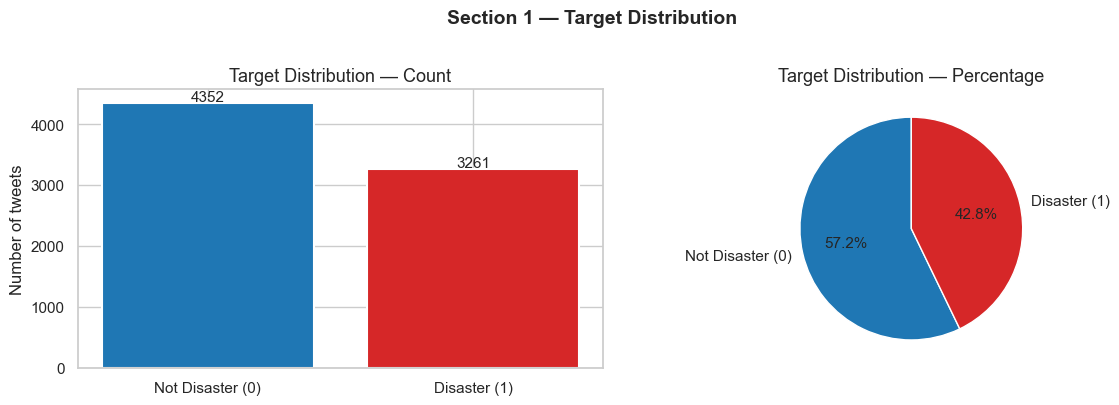
\includegraphics[width=0.45\textwidth]{images/eda_01_target_distribution.png}
    \caption{Class distribution in the training set.}
    \label{fig:target_dist}
\end{figure}

\subsection{Exploratory Data Analysis}
Meta-feature analysis reveals systematic differences between the two classes. Disaster tweets are on average longer (108.3 characters vs 95.8) and use longer words (mean word length 6.47 vs 5.87), consistent with the hypothesis that disaster-related content originates more frequently from news agencies writing in formal register, while non-disaster tweets come from individual users using informal language. Keyword analysis confirms this signal: keywords such as \textit{debris}, \textit{derailment}, and \textit{wreckage} have a disaster rate above 95\%, while \textit{body-bags} and \textit{aftershock} have rates below 3\% — indicating strong metaphorical or colloquial use. These observations directly motivate the use of contextual embeddings, which can disambiguate the same keyword across different linguistic contexts. Fig.~\ref{fig:meta} shows the distribution of selected meta-features by class.

\begin{figure}[h]
    \centering
    
\includegraphics[width=0.48\textwidth]{images/eda_03_meta_features.png}
    \caption{Meta-feature distributions by class (top row only).}
    \label{fig:meta}
\end{figure}

Train and test sets share nearly identical meta-feature distributions (e.g., mean word count 14.90 vs 14.97), confirming that both sets are drawn from the same underlying population and that no distribution shift is expected at inference time.

\subsection{Mislabeled Samples Correction}

The training set contains 18 tweets that appear multiple times with contradictory labels, assigned by different crowdworkers who interpreted ambiguous content differently~\cite{evitan2020mislabeled}. Examples include religious references to \textit{Hellfire}, metaphorical uses of \textit{burning buildings}, and borderline safety warnings such as \textit{``Caution: breathing may be hazardous to your health.''} Retaining these conflicting duplicates would introduce noise directly into the training signal. We identified them by grouping tweets by text and flagging those with more than one unique target value, then manually assigned the correct label by reading each tweet in context, storing the result in a dedicated \texttt{target\_relabeled} column to preserve the original annotations.

\subsection{Text Cleaning and Preprocessing}

Raw tweets require extensive cleaning before tokenization. Following~\cite{evitan2020mislabeled}, we apply a multi-step pipeline: URLs are removed, character encoding artifacts (e.g., \texttt{\textbackslash x89Ûª}) are stripped, contractions are expanded (\textit{can't} $\rightarrow$ \textit{cannot}), punctuations are separated from words to improve embedding coverage, and common typos and slang are normalised. Compound hashtags and informative usernames (e.g., \texttt{NASAHurricane} $\rightarrow$ \textit{NASA Hurricane}) are expanded into readable tokens, since concatenated words lack embeddings in both GloVe and BERTweet vocabularies. This cleaning step is applied consistently to both training and test sets before any modelling step. Prior to any preprocessing step, missing values in the \texttt{keyword} and \texttt{location} columns were filled with a placeholder string (\texttt{no\_keyword}, \texttt{no\_location}) to avoid downstream errors in feature extraction. No missing values were found in the \texttt{text} column.

\subsection{Data Augmentation via Back-Translation}

Since we are utilizing Transformer-based models, the available training data may be insufficient for the model to learn its weights efficiently. Data augmentation for raw text is notoriously difficult compared to computer vision; while an image can be rotated or flipped without losing its meaning, text is fragile. To address this, we implemented a back-translation pipeline. We first translate the English source text into a linguistically distant language—in our case, Hindi—and then translate it back into English. Because Hindi employs a different script (Devanagari) and distinct grammatical structures, the resulting English output often retains the original sentiment and semantics but utilizes varied syntax and synonyms. This process teaches the model that different linguistic paths can lead to the same conceptual destination, effectively increasing the diversity of our dataset. The interaction between this augmentation strategy and the chosen fine-tuning approach is discussed in Section \ref{subsec:dataaugmentation} in light of experimental results. The augmented set doubled the training data to $\sim$15{,}000 samples.

% =============================================================================
% III. MODELING APPROACH
% =============================================================================

\section{Modeling Approach}

The overall architecture of our proposed system, from raw data ingestion to final inference, is illustrated in Fig.~\ref{fig:pipeline_snake_compact}. The pipeline consists of five main phases: data preprocessing, augmentation, architecture selection, model training, and final inference. Each phase is detailed in the following subsections.

% === ULTRA-COMPACT SNAKE-LAYOUT PIPELINE ===
\begin{figure}[htbp]
    \centering
    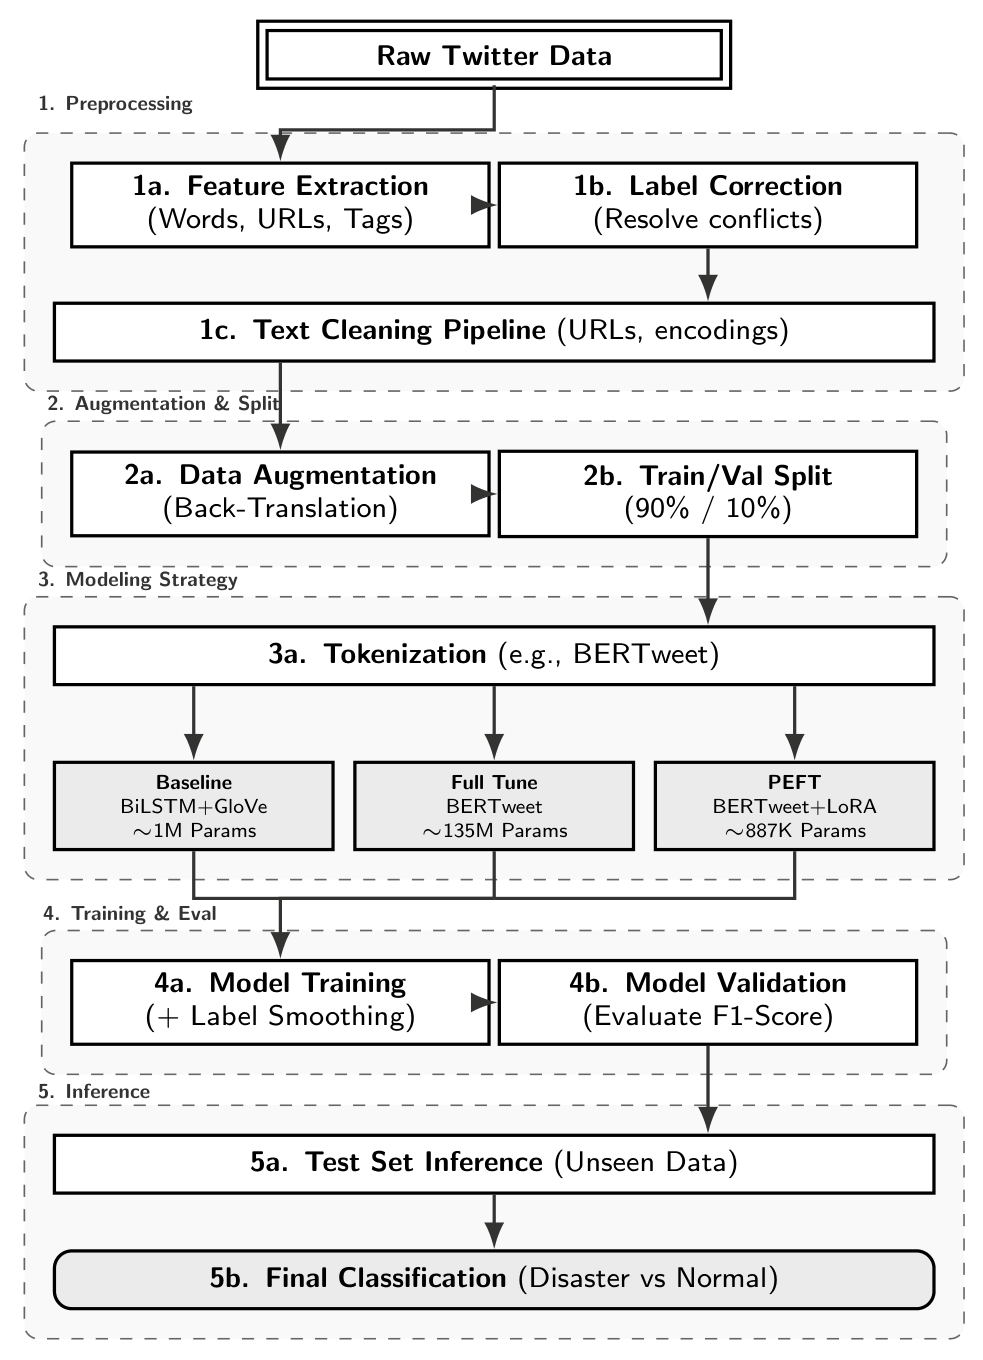
\includegraphics[width=0.6\columnwidth]{images/tikz-1.png}
    \caption{End-to-end pipeline for disaster tweet classification.}
    \label{fig:pipeline_snake_compact}
\end{figure}

\subsection{Start Point: Machine Learning (Non-Deep) Approach}

As a non-deep lower bound, we first evaluate a TF-IDF representation combined with Logistic Regression~\cite{tunguz_tfidf_kaggle}. This approach treats each tweet as a bag of words, discarding word order and context entirely. As noted in the literature, deep learning is not always a silver bullet~\cite{silver_bullet_nlp}: simpler models can be bcompetitive on small, well-curated datasets, and their limitations must be demonstrated empirically before introducing more complex architectures. TF-IDF + Logistic Regression achieves a validation F1 of 0.730 and a Kaggle F1 of 0.791 — clearly below BiLSTM (0.810) and Transformer-based models. This confirms that bag-of-words representations are insufficient for this task, without word order or contextual information, the model cannot disambiguate identical keywords used in both literal and metaphorical contexts, directly motivating the use of sequential and contextual models.

\subsection{Why Transformers for this Task}
Transformers truly shine when there is a strong language component in the problem, and specifically when one can exploit the ambiguity and richness of natural language. Outside of that domain, their use should be carefully justified. Transformers compute contextual representations in which the same token receives a different embedding depending on its surrounding words, making them naturally suited to resolving this kind of lexical ambiguity. Twitter text is characterised by abbreviations, hashtags, and informal language that fall outside the distribution of standard English corpora. BERTweet~\cite{nguyen2020bertweet}, pre-trained on 850 million English tweets, aligns model vocabulary and pre-training distribution with the target domain, making it a more suitable choice than generic alternatives such as BERT~\cite{devlin2019bert}.

\subsection{Baseline: BiLSTM with GloVe Embeddings}
As a baseline for disaster tweet classification, we implemented a recurrent architecture combining pre-trained GloVe \cite{nikjohn7_kaggle} embeddings with bidirectional LSTMs \cite{akashkr_kaggle}. This setup captures semantic and sequential patterns in short, noisy text. The architecture starts with a foundational layer of \textbf{GloVe (Global Vectors for Word Representation)} embeddings \cite{pennington2014glove}. We utilized 100-dimensional vectors pre-trained on a 6-billion token corpus (Wikipedia + Gigaword). To prevent overfitting on the relatively small training set ($\sim$7k samples), the embedding layer was kept \textbf{frozen}, acting as a robust feature extractor that provides semantic regularities for free \cite{akashkr_kaggle}. The core of the model consists of \textbf{Bidirectional LSTM (BiLSTM)} layers. Unlike standard LSTMs, BiLSTMs process sequences in both directions, concatenating hidden states to capture the full context of a tweet \cite{akashkr_kaggle}. This is critical for disaster detection, where key terms (e.g., "fire", "flood") may appear at any position. Research shows that BiLSTMs consistently outperform traditional Bag-of-Words and TF-IDF methods by modeling long-term dependencies and word relationships across time steps \cite{nikjohn7_kaggle}. The final output layer uses a single neuron with Sigmoid activation for binary classification, consistent with the Kaggle task \cite{kaggle}.

\subsection{BERT Fine-Tuning}
Fine-tuning is the process of adapting a pre-trained model to solve a specific problem using target data, making state-of-the-art deep learning accessible without the need for massive computational resources \cite{prof_lecture}. To adapt BERT for our binary classification task, we add a task-specific output layer on top of the pre-trained architecture and update all the model parameters jointly \cite{sun2019how}. This end-to-end training allows the model to tailor its deep, contextual understanding of language directly to our domain, maximizing task-specific performance within our domain \cite{medium_bert}. In our experiments, we fine-tuned the \texttt{bert-base-uncased} model ($\sim$110M parameters) as a general-purpose Transformer baseline. The model was trained for 3 epochs with a learning rate of \texttt{2e-5} and a 10\% warmup ratio to ensure stability during the initial phase of optimization.

\subsection{BERTweet: Domain-Specific Pre-Training}
BERTweet shares the same architecture as BERT-base, but it’s pretrained like RoBERTa on English Tweets. It achieves strong performance on Tweet-related tasks like part-of-speech tagging, named entity recognition, and text classification \cite{huggingface_bertweet}. The discovery of BERTweet as a specialized architecture for this task was prompted by community benchmarks \cite{tripathi_bertweet_kaggle}, which highlighted the limitations of general-purpose models when dealing with the idiosyncratic nature of social media language. As described by Nguyen et al. \cite{nguyen2020bertweet}, BERTweet is the first large-scale pre-trained language model for English Tweets, designed to bridge the gap between formal corpora (like Wikipedia or News) and the informal, noise-heavy characteristics of microblogging data. The model adopts the same architecture as BERT-base and follows the RoBERTa pre-training procedure \cite{nguyen2020bertweet}. It was trained on a massive 80GB corpus comprising 850M English Tweets (approximately 16B tokens). Specifically, the authors report that BERTweet achieves superior performance in text classification, producing state-of-the-art results on benchmark datasets like SemEval2017 Task 4A and SemEval2018 Task 3A \cite{nguyen2020bertweet}. In the context of disaster tweet classification, this specialization is critical for correctly interpreting hashtags, slang, and the frequent use of informal grammar that characterizes our dataset.

\subsection{Parameter-Efficient Fine-Tuning with LoRA}
To address computational overhead and the risk of overfitting on a relatively small training dataset, we implemented Parameter-Efficient Fine-Tuning (PEFT), specifically focusing on Low-Rank Adaptation (LoRA)\cite{hu2021lora}. Unlike traditional full fine-tuning, which updates all approximately 135 million parameters of the BERTweet architecture, LoRA freezes the original pre-trained weights and injects small, trainable rank-decomposition matrices into the model's attention layers. Mathematically, for a given weight matrix $W$, the update is represented as $W' = W + BA$, where $B$ and $A$ are low-rank matrices. LoRA's rank configuration enables reducing the number of trainable parameters to a fraction of a percent compared to the totality updated in full fine-tuning. This efficiency stands in stark contrast to both full fine-tuning, which updates 100\% of the Transformer's parameters, and our baseline BiLSTM model, which also requires training 100\% of its approximately 1 million parameters. This massive reduction not only accelerates training and decreases memory usage, but also serves as an effective regularizer to mitigate overfitting risks on social media text.

\subsection{DoRA: Weight-Decomposition Low-Rank Adaptation}
DoRA (Weight-Decomposition Low-Rank Adaptation) is an evolution of LoRA that decomposes the pre-trained weight matrix into two distinct components: \textbf{magnitude} and \textbf{direction} \cite{prof_lecture, liu2024dora}. While standard LoRA updates both simultaneously through low-rank matrices, DoRA decouples them, allowing the model to learn directional updates ($D$) via low-rank adaptation while explicitly tuning a trainable magnitude vector ($m$) \cite{prof_lecture}. Theoretically, this addresses LoRA's limitation in capturing magnitude changes independently, potentially leading to superior performance on complex tasks \cite{liu2024dora}. However, empirical evidence suggests that DoRA's theoretical superiority does not always translate into higher accuracy across all tasks. On simpler datasets or architectures, the added complexity of learning separate magnitude parameters can result in slower convergence or even performance lag compared to the simpler LoRA framework \cite{ullah2025lora}.

\subsection{Label Smoothing and Regularization}

Label smoothing~\cite{szegedy2016rethinking} replaces hard targets $\{0, 1\}$ with soft targets $\{\varepsilon/2,\, 1-\varepsilon/2\}$, preventing the model from becoming overconfident on ambiguous samples. This is particularly relevant in our setting: even after manually correcting 18 mislabeled samples, some tweets remain genuinely ambiguous due to metaphorical use of disaster-related keywords.
% =============================================================================
% IV. RESULTS
% =============================================================================

\section{Results}

\subsection{Evaluation Metric}
Performance is evaluated using the binary F1-score, consistent with the Kaggle competition metric. Accuracy would be misleading on an imbalanced dataset, as a model predicting the majority class could still achieve high accuracy while performing poorly on the minority class. F1-score balances precision and recall, penalising both false positives (incorrectly flagging a non-disaster tweet) and false negatives (missing a real disaster event). This is important in our context, since both missing a real disaster (false negative) and incorrectly flagging a non-disaster tweet (false positive) can negatively impact the usefulness of the system.

\subsection{Model Comparison}

Table~\ref{tab:results} summarises the results across all models. Notably, BERTweet + LoRA achieves the best Kaggle F1 while training only 0.65\% of the total parameters, outperforming full fine-tuning approaches with orders of magnitude more trainable weights.

\begin{table}[h]
\centering
\caption{Results on the Kaggle public leaderboard.
         The best score is highlighted in \textbf{bold}.}
\label{tab:results}
\resizebox{\columnwidth}{!}{%
\begin{tabular}{lccc}
\toprule
Model & Val F1 & Kaggle F1 & Params \\
\midrule
TF-IDF + Logistic Regression
    & 0.730 & 0.791 & — (non-deep) \\
BiLSTM + GloVe 100d
    & 0.776 & 0.810 & $\sim$1M (100\%) \\
BERT fine-tuning
    & 0.829 & 0.834 & $\sim$110M (100\%) \\
BERTweet fine-tuning
    & 0.821 & 0.839 & $\sim$135M (100\%) \\
\textbf{BERTweet + LoRA} (r=8)
    & \textbf{0.813} & \textbf{0.847} & \textbf{887K (0.65\%)} \\
BERTweet + DoRA (r=16)
    & 0.811 & 0.841 & 1.2M (0.90\%) \\
BERTweet-large fine-tuning
    & 0.812 & 0.844 & $\sim$355M (100\%) \\
BERTweet-large + LoRA (r=16)
    & 0.811 & 0.841 & 8M (2.24\%) \\
\bottomrule
\end{tabular}%
}
\end{table}

\subsection{Key Findings}

Our experimental evaluation yielded several critical insights regarding the interplay between parameter capacity, regularization, and data augmentation in domain-specific language models.

\textbf{LoRA outperforms full fine-tuning with a fraction of parameters.}
Our baseline BERTweet model, fully fine-tuned for 3 epochs at \texttt{lr=2e-5} with warmup~\cite{devlin2019bert}, utilizes all $\sim$135M parameters to achieve a Kaggle F1-score of 0.839. LoRA~\cite{hu2021lora} with rank $r=8$ — the default recommended in the original paper as sufficient for most NLP classification tasks — reduces the trainable footprint to just 887,042 weights (0.65\%), while achieving a superior Kaggle F1-score of 0.847.

\textbf{DoRA does not improve over LoRA on this domain.}
Our DoRA~\cite{liu2024dora} implementation used rank $r=16$ to compensate for the added complexity of decoupling magnitude and direction, yet reached only 0.841. This confirms that LoRA's simplicity acts as a more effective regularizer on this domain~\cite{ullah2025lora}: DoRA's magnitude component appears to require more training epochs or higher-signal data to fully realize its theoretical potential.

\textbf{Domain-specific pre-training generalizes better than BERT.}
BERTweet outperformed standard BERT by 0.005 on the Kaggle leaderboard. Despite BERT achieving a higher validation score, BERTweet's pre-training on 850M tweets proved more effective at generalizing to the informal and noisy language of disaster-related microblogging.

\textbf{Label smoothing benefits parameter-constrained models.}
Applying a smoothing factor of $\varepsilon = 0.1$ yielded a consistent improvement of $+0.002$ F1 on the Kaggle leaderboard for LoRA-based models~\cite{ullah2025lora}, while the same parameter slightly degraded the fully fine-tuned BERTweet model~\cite{medium_bert}. This confirms that explicit regularization is most beneficial when the number of trainable parameters is strictly limited.

\textbf{Back-translation augmentation hurts LoRA but helps
full fine-tuning.}
Augmented data acted as a regularizer for full fine-tuning, whose massive parameter space is prone to overfitting on small datasets. Conversely, it degraded LoRA performance: because low-rank matrices have limited capacity, every training sample must carry a strong signal. The semantic drift and grammatical noise introduced by back-translation effectively polluted LoRA's trainable parameters, yielding a less precise model than one trained on the original, unaugmented data alone.

\subsection{Effect of Data Augmentation on Fine-Tuning Strategy}
\label{subsec:dataaugmentation}
While data augmentation is a staple in deep learning, its effectiveness varies significantly depending on the fine-tuning strategy. In Full Fine-Tuning, every parameter in the model is updated ($W = W_0 + \Delta W$). Because the model has a massive degree of freedom, it is prone to overfitting on small, repetitive datasets. Augmentation acts as a regularizer. By providing back-translated variations, the model is forced to learn generalized features rather than memorizing specific patterns or "noise" in the original training set. It expands the decision boundary, making the model more robust. LoRA freezes the original weights and only trains a small pair of rank-decomposition matrices. The update is represented as: $\Delta W = BA$ where $B$ and $A$ are low-rank matrices. LoRA is designed to be parameter-efficient. It excels at learning specific tasks or styles from high-quality, "clean" data. If the back-translation process introduces even slight semantic drift or grammatical "hallucinations" (a common side effect of translation models), LoRA may capture this noise as a primary signal. Because the rank (capacity) of LoRA is limited, every training sample must be high-signal. Low-quality augmented data can "pollute" the small number of trainable parameters, leading to a model that is less precise than one trained on a smaller, pristine dataset.

% =============================================================================
% V. CONCLUSION
% =============================================================================

\section{Conclusion}
In this study, we explored a progressive series of NLP architectures for disaster tweet classification, from a recurrent BiLSTM baseline  to domain-specific Transformers with parameter-efficient fine-tuning. Domain-specific pre-training (BERTweet) proved more effective than  general-purpose BERT at capturing the informal, noisy nature of social  media language. More strikingly, PEFT via LoRA demonstrated that  drastically reducing the number of trainable parameters not only cuts  computational cost, but can actually improve generalization —  outperforming full fine-tuning on this domain. While our results are robust, the disambiguation of metaphorical language remains an open challenge. Future research could integrate sentiment and emotion analysis to further refine classification, as the underlying intent of a tweet often provides critical context for disaster detection \cite{mahalavanya_github}. Future work could explore two promising directions: multimodal classification, incorporating images attached to tweets alongside text~\cite{basit2023multimodal}; and semi-supervised learning, leveraging the large volume of unlabelled social media data to reduce dependence on hand-annotated samples~\cite{popovici2025multihead}. Overall, participating in this Kaggle competition was an enlightening experience that allowed us to apply state-of-the-art NLP methods to a real-world classification task under computational constraints. The complete  codebase is publicly available at~\cite{our_github}.

% =============================================================================
% VI. Use of AI Assistance
% =============================================================================

\section{Use of AI Assistance}

AI tools were used as an accelerator for development, not as a replacement for critical thinking. Every architectural decision, experimental choice, and line of code was understood, validated, and intentionally included by the team. 
The primary use of AI was to systematically scan external Kaggle notebooks and research papers, surfacing implementation details that are easy to overlook. Two concrete examples: AI flagged the use of a warmup scheduler (\texttt{warmup\_ratio=0.1}) as a training stability improvement, applied consistently across all Transformer notebooks; and identified that 
\texttt{finiteautomata/bertweet-base-sentiment-
analysis} was built on \texttt{vinai/bertweet-base}~\cite{tripathi_bertweet_kaggle}, leading to the adoption of BERTweet as our final model. Decisions such as filtering augmented rows from validation, correcting 18 mislabeled samples, and applying back-translation augmentation were made entirely by the team. AI accelerated execution without compromising the  integrity of the research process.

% =============================================================================
% REFERENCES
% =============================================================================

\begin{thebibliography}{00}

\bibitem{kaggle}
A. Howard, devrishi, P. Culliton, and Y. Guo,
``Natural Language Processing with Disaster Tweets,''
Kaggle, 2019.
\url{https://kaggle.com/competitions/nlp-getting-started}

\bibitem{devlin2019bert}
J. Devlin, M.-W. Chang, K. Lee, and K. Toutanova,
``BERT: Pre-training of Deep Bidirectional Transformers for Language
Understanding,''
\textit{arXiv preprint arXiv:1810.04805}, 2019.

\bibitem{nguyen2020bertweet}
D. Q. Nguyen, T. Vu, and A. T. Nguyen,
``BERTweet: A pre-trained language model for English Tweets,''
\textit{arXiv preprint arXiv:2005.10200}, 2020.

\bibitem{hu2021lora}
E. J. Hu et al.,
``LoRA: Low-Rank Adaptation of Large Language Models,''
\textit{arXiv preprint arXiv:2106.09685}, 2021.

\bibitem{liu2024dora}
S.-Y. Liu et al.,
``DoRA: Weight-Decomposed Low-Rank Adaptation,''
\textit{arXiv preprint arXiv:2402.09353}, 2024.

\bibitem{pennington2014glove}
J. Pennington, R. Socher, and C. D. Manning,
``GloVe: Global Vectors for Word Representation,''
in \textit{Proc. EMNLP}, 2014.

\bibitem{szegedy2016rethinking}
C. Szegedy et al.,
``Rethinking the Inception Architecture for Computer Vision,''
in \textit{Proc. CVPR}, 2016.

\bibitem{tripathi_bertweet_kaggle}
D. Tripathi,
``EDA, Data Augmentation and Prediction with RoBERTa and cTF-IDF,''
Kaggle Notebook, 2021.
\url{https://www.kaggle.com/code/deepaktripathiuk/eda-data-augment-predict-with-roberta-n-ctf-idf}

\bibitem{evitan2020mislabeled}
G. Evitan,
``NLP with Disaster Tweets — EDA, Cleaning and BERT,''
Kaggle Notebook, 2020.
\url{https://www.kaggle.com/code/gunesevitan/nlp-with-disaster-tweets-eda-cleaning-and-bert}

\bibitem{huggingface_bertweet}
``BERTweet''
Hugging Face, 2020.
\url{https://huggingface.co/docs/transformers/model_doc/bertweet}

\bibitem{nikjohn7_kaggle}
N. John,
``Disaster-Tweets-Kaggle: Meaningful Vector Representation using GloVe,''
GitHub Repository, 2020.
\url{https://github.com/nikjohn7/Disaster-Tweets-Kaggle}

\bibitem{akashkr_kaggle}
A. Kumar,
``TF-Keras Tutorial: Bi-LSTM, GloVe, GRU,''
Kaggle Notebook, 2021.
\url{https://www.kaggle.com/code/akashkr/tf-keras-tutorial-bi-lstm-glove-gru-part-6}

\bibitem{our_github}
S. P. Candido, A. Gaudino, D. Gosmar, and A. Kallas, 
``NLP with Disaster Tweets: From Sequential Models to Parameter-Efficient Transformers,'' 
GitHub Repository, 2024. [Online]. Available: \url{https://github.com/andreaGaudino/NLP_with_disaster_tweets}

\bibitem{mahalavanya_github}
M. Sriram, ``Natural Language Processing with Disaster Tweets,'' 
GitHub Repository, 2020. [Online]. Available: \url{https://github.com/MahalavanyaSriram/Natural-Language-Processing-with-Disaster-Tweets}

\bibitem{prof_lecture}
EURECOM, ``Convolutional Neural Networks,'' Deep Learning Course, 2026. [Online]. Available: \url{https://eurecom-ds.github.io/deeplearning/editions/2026/slides/conv_nets.html#/title-slide}

\bibitem{sun2019how}
C. Sun, X. Qiu, Y. Xu, and X. Huang, ``How to Fine-Tune BERT for Text Classification?,'' \textit{arXiv preprint arXiv:1905.05583}, 2019.

\bibitem{medium_bert}
A. Amit, ``Fine-tuning BERT for Classification: A Practical Guide,'' Medium, 2023. [Online]. Available: \url{https://medium.com/@heyamit10/fine-tuning-bert-for-classification-a-practical-guide-b8c1c56f252c}

\bibitem{ullah2025lora}
I. Ullah, ``LoRA vs DoRA on MNIST: When Theory Meets Reality,'' Medium, 2025. [Online]. Available: \url{https://imranullahds.medium.com/lora-vs-dora-on-mnist-when-theory-meets-reality-be277176c2ea}

\bibitem{basit2023multimodal}
M. Basit, B. Alam, Z. Fatima, and S. Shaikh,
``Natural Disaster Tweets Classification Using Multimodal Data,''
in \textit{Proc. Conference on Empirical Methods in Natural Language
Processing (EMNLP)}, Singapore, Dec. 2023, pp. 7584--7594.

\bibitem{popovici2025multihead}
R.-A. Popovici and T. Rebedea,
``Multihead Average Pseudo-Margin Learning for Disaster Tweet
Classification,''
\textit{Information}, vol. 16, no. 6, p. 434, May 2025.

\bibitem{tunguz_tfidf_kaggle}
B. Tunguz,
``Twitter Disaster with TF-IDF and LR,''
Kaggle Notebook, 2020.
\url{https://www.kaggle.com/code/tunguz/twitter-disaster-with-tf-idf-and-lr/notebook}

\bibitem{silver_bullet_nlp}
``Deep Learning May Not Be the Silver Bullet for All NLP Tasks Just Yet,''
Towards Data Science, 2019.
\url{https://towardsdatascience.com/deep-learning-may-not-be-the-silver-bullet-for-all-nlp-tasks-just-yet-7e83405b8359/}

\end{thebibliography}

\end{document}
